\documentclass[12pt]{article}
\usepackage[utf8]{inputenc}
\usepackage{geometry, setspace}
\geometry{a4paper, portrait, margin=1in}
\usepackage{amsmath}
\usepackage{graphicx}
\usepackage{float}
\usepackage{minted}
\usepackage{hyperref}
\usepackage{setspace}
\usepackage{caption, subcaption}
\usepackage[title]{appendix}
\usepackage{booktabs, tabularx}
\usepackage{tikz}
\usepackage{latexsym}
% \usepackage{indentfirst}
\hypersetup{
    colorlinks,
    citecolor=black,
    filecolor=black,
    linkcolor=black,
    urlcolor=black
}

\newtheorem{definition}{Definition}
\newtheorem{lemma}{Lemma}
\newenvironment{proof}{\par\noindent{\it Proof.}\hspace*{1em}}{$\Box$\bigskip}

\begin{document}
% --------- title page -------------
\begin{titlepage}
    \begin{center}
        \vspace*{1cm}
 
        \LARGE\textbf{Near-Optimal Concurrent Events Rendering by Graph Coloring and DFS}
   
        \vspace{1.5cm}
 
        \textbf{Hanzhi Zhou}
 
        \vfill
        \vspace{0.8cm}

        \Large
        School of Engineering and Applied Science\\
        \vspace{0.2cm}
        University of Virginia\\
        \vspace{0.2cm}
        \today
        \vspace{1cm}
    \end{center}
    \clearpage
\end{titlepage}

\section{Introduction}
\begin{figure}[H]
    \centering
    \includegraphics[width=.8\columnwidth]{example-event.png}
    \caption{Example events}
    \label{fig:ev-exp-1}
\end{figure}

\begin{definition}
    \textbf{Time period} of an event is defined as the (\textbf{start time}, \textbf{end time}), where \textbf{start time} and \textbf{end time} are measured in terms of the number of minutes after 0:00.
\end{definition}

\begin{definition}
    \textbf{width} of an event is defined as the width of the rectangle block containing the event divided by the width of the column. 
\end{definition}

\begin{definition}
    \textbf{left} of an event is defined as the distance between the left border of the event and the left border of the column divided by the width of the column.
\end{definition}

As an example, the time periods, width and left of the two events shown in Figure~\ref{fig:ev-exp-1} are listed in Table~\ref{tab:ev-param}.
\begin{table}[H]
    \centering
    \caption{Event rendering parameters}\label{tab:ev-param}
    \begin{tabular}{cccc}
        \toprule
        Event Name & Time Period & Width & Left \\
        \midrule
        CS 2102 & (480, 555) & 0.5 & 0 \\
        Example Event & (480, 555) & 0.5 & 0.5 \\
        \bottomrule
    \end{tabular}
\end{table}

\begin{lemma}
    An event can be rendered by knowing the \textbf{time period}, \textbf{width} and \textbf{left}.
\end{lemma}
\begin{proof}
    An event on a schedule is nothing more than a rectangle on a grid. Time periods define the start and end of the event, which can be converted to top and height. With width and left also defined, such rectangle is unique.
\end{proof}

The time period is a known parameter for each event. Therefore, the main focus is the calculation of width and left.

\section{Graph Representation}
\begin{figure}[H]
    \centering
    \begin{subfigure}{.4\textwidth}
        \centering
        \includegraphics[width=.9\columnwidth]{example1}
        \caption{A Simple Schedule}
        \label{fig:exp1}
    \end{subfigure}%
    \begin{subfigure}{.6\textwidth}
        \centering
        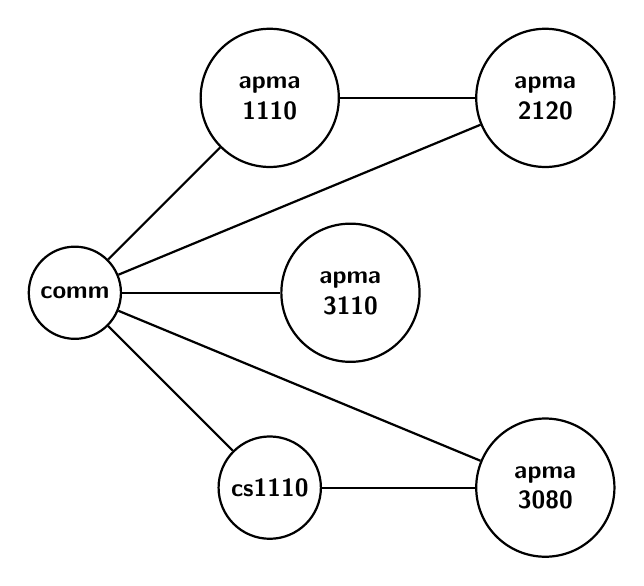
\begin{tikzpicture}[auto, node distance=3.5cm, every loop/.style={},
            thick,main node/.style={circle,draw,font=\sffamily\bfseries\small}]
        
        \node[main node] (comm) {comm};
        \node[main node] (apma1110) [above right of=comm] {\begin{tabular}{c}
            apma \\ 1110
        \end{tabular}};
        \node[main node] (apma2120) [right of=apma1110] {\begin{tabular}{c}
            apma \\ 2120
        \end{tabular}};
        \node[main node] (apma3110) [right of=comm] {\begin{tabular}{c}
            apma \\ 3110
        \end{tabular}};
        \node[main node] (cs1110) [below right of=comm] {cs1110};
        \node[main node] (apma3080) [right of=cs1110] {\begin{tabular}{c}
            apma \\ 3080
        \end{tabular}};

        \path[every node/.style={font=\sffamily\small}]
        (comm) edge node { } (apma1110)
        (comm) edge node { } (apma2120)
        (comm) edge node { } (apma3110)
        (comm) edge node { } (apma3080)
        (apma1110) edge node { } (apma2120)
        (cs1110) edge node { } (apma3080)
        (comm) edge node { } (cs1110);
        \end{tikzpicture}
        \caption{Graph Representation}
        \label{fig:graphexp1}
    \end{subfigure}%
    \caption{}
    \label{}
\end{figure}

\begin{definition}
    Two events are said to be \textbf{conflicting} iff the time periods in which they take place have overlap.
\end{definition}

\begin{definition}
    Slots are positions in a column that contain events. They are uniquely identified by their \textbf{left}. All slots have equal width. An event occupies at least one slot. 
\end{definition}

The main principle behind schedule rendering is that two conflicting events cannot share the same slot, otherwise there must be a part where they appear to overlap with one another.
The k-colorability problem asks whether it is possible to color the vertices of a graph using k colors, subject to the condition that no two adjacent nodes have the same color. We can slightly modify the problem statement so its applicable to our problem: given a set of events, some of which may have conflicts, is it possible to allocate k \textbf{slots} such that no two adjacent (conflicting) events occupy the same \textbf{slot}.

From our new problem statement, we arrive at the graph representation of the set of events that we want to render.

\begin{definition}\label{def:3}
    Each event is represented as a \textbf{node (vertex)}, and every two nodes are connected by an edge iff they have conflict.
\end{definition}

Using definition~\ref{def:3}, we can construct a graph for the set of events shown in Figure~\ref{fig:exp1}. The resulting graph is shown in Figure~\ref{fig:graphexp1}.

\section{Graph Coloring Algorithm}
Graph coloring is an NP-complete problem, which means there is no known algorithm that can solve it in polynomial time. The exact algorithm (algorithm that is able to find the optimal solution) using the backtrack approach still takes exponential time. 

Nevertheless, approximation algorithms such as Degree of Saturation (DSATUR) can find a reasonably good solution for our problem. DSATUR can also provide a good initial ordering of the vertices to be colored for the backtrack algorithm. There are better graph coloring approximation algorithm such as the recursive largest first (RLF) algorithm, but for small graphs, DSATUR plays almost equally well. For simplicity, we used DSATUR to provide the initial vertex ordering for the backtrack algorithm, with forced-breaking when the number of recursive calls exceeds $10^6$. For small graphs, this 0method provides almost exact solutions.

\section{Position Calculation}
Even if the coloring of our graph is obtained, there is some extra work involved in turning the colors to positions.

\subsection{Naive Approach}
\begin{figure}[H]
    \centering
    \includegraphics[width=\columnwidth]{pos-calc-exp1.png}
    \caption{Position Calculation: A Naive Approach}
    \label{fig:pos-naive}
\end{figure}
After the coloring is obtained, a naive approach to turn colors into left and width, given that colors are represented as integers starting from 0, is
\begin{align*}
    \text{left} &= \frac{\text{color of this event}}{\text{total number of colors}} \\
    \text{width} &= \frac{1}{\text{total number of colors}}
\end{align*}

However, this method does not give a satisfying result. Figure~\ref{fig:pos-naive} demonstrates its problem: Some events are not `aware' of the fact that there is no event of greater color after it and that it can have `extended' width. For example, `APMA 3110' has color 1, but there is no node that has color 2 adajcent to it, so it can actually have twice the width as `COMM 3010' which has color 0. To solve this problem, we developed a method explained in the next section. 

\subsection{Color DFS}
To deal with the problem of the naive approach, we developed a DFS-based method to discover the maximum depth of the path that each node is on. Our algorithm is slightly different from the conventional DFS due to the fact that the depth of all nodes are known beforehand. 

\end{document}